\chapter{Infrastruktur}
\label{infrastruktur}

\section{Architektur}

Das Gesamtsystem setzt sich aus insgesamt vier Komponenten zusammen: die Datenbank, der Webserver, die Fehlerquelle und das Zielsystem von OpenStreetMap. 
Die einzelnen Komponenten sind über \gls{REST}-Schnittstellen miteinander verbunden. 
Dabei sind das Zielsystem (OpenStreetMap) und die Fehlerquelle (Keepright, siehe Kapitel \ref{datenquellen}) Fremdsysteme, bei welchen die Schnittstellen gegeben waren. 
Unsere eigenen Server haben wir entsprechend angepasst und auch via REST zugänglich gemacht.

\begin{figure}[H]
	\centering
	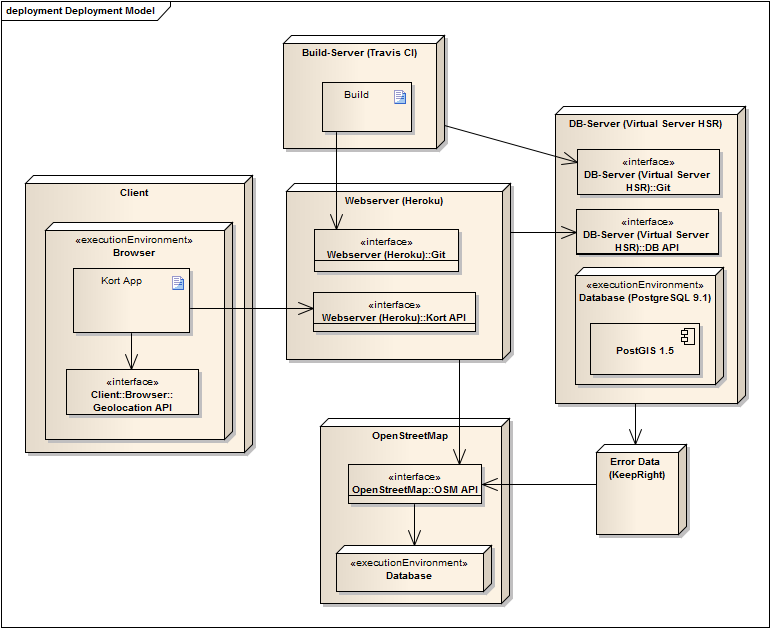
\includegraphics[width=\textwidth]{images/uml/deployment_diagram}
	\caption{Gesamtübersicht der Systeme}
	\label{deplyoyment-diagram}
\end{figure}


\section{Datenbankserver}

Beim Datenbankserver handelt es sich um einen virtuellen Server, den uns die Hochschule für Technik Rapperswil (HSR) zur Verfügung gestellt hat für die Dauer dieser Arbeit.
Dieser Server hält die Installation der \textsc{Kort}-Datenbank sowie das Projektmanagementtool Redmine.
Letzteres ist die einzige kritische Anwendung auf dem Server, da der Rest sich über entsprechende Installationskripts sehr einfach und schnell neu aufbauen lässt.

Die Installation der benötigten Software kann mit dem Ubuntu Standard-Mechanismus \inlinecode{apt-get install} durchgeführt werden.


\begin{table}[H]
\centering
\begin{tabular}{|p{0.25\twocelltabwidth}|p{0.75\twocelltabwidth}|}
\hline 
\small{\textbf{Name}} & sinv-56055.edu.hsr.ch \\
\hline
\small{\textbf{DNS CNAME}} & kort.rdmr.ch \\
\hline 
\small{\textbf{Art des Servers}} & Virtueller Server \\
\hline 
\small{\textbf{Betriebsystem}} & Ubuntu 12.04 (LTS) \\
\hline 
\small{\textbf{Zugriff}} & Root-Zugriff via SSH \\
\hline 
\small{\textbf{Installierte Software}} & PostgreSQL 9.1, PostGIS 2.0, Redmine 2.1, MySQL 5.5, Apache Websever mit PHP 5.4 \\
\hline 
\small{\textbf{Pfade}} & Repository: \inlinecode{/home/odi/kort} \\
Redmine: \inlinecode{/home/redmine/redmine-2.1.0} \\
\hline 
\end{tabular} 
\caption{Datenbankserver der Hochschule für Technik Rapperswil}
\label{infrastruktur-datenbankserver-tabelle}
\end{table}

\subsection{Datenbank-Webservice}
Der Zugang auf die Datenbank von aussen läuft ausschliesslich über den REST-Webservice.
Für den Betrieb dieses Dienstes ist eine Apache Webserver Installation mit PHP-Unterstützung (mindestens PHP 5.3) erforderlich.

Für den Betrieb der Webservice ist das \textsc{Kort}-Repository auf dem Server geklont.
Anschliessend muss noch ein Symlink angelegt werden um das Skript korrekt aufrufen zu können:

\inlinecode{\$ ln -s /home/odi/kort/server/webservices /var/www/webservices}

Damit der der REST-Endpunkt auf der Datenbank-Server unter der Adresse \url{http://kort.rdmr.ch/webservices/db} erreichbar.

\subsection{Redmine}
Die Installation von Redmine verlangt es, einen neuen Benutzer \inlinecode{redmine} auf dem Server anzulegen.
Danach muss die Software nur noch auf den Server kopiert werden und der Installationsanleitung gefolgt werden.
Diese ist in unserem Repository zu finden: \url{https://github.com/odi86/kort/blob/master/server/redmine/redmine_install.md}

\subsubsection{Backup}
Die Daten von Redmine werden über 2 Skripts täglich gesichert. 
Das Skript \inlinecode{ŕedmine\_backup.sh} kümmert sich darum alle Backup-Daten täglich auf dem virtuellen Server zu sammeln und an einem zentralen Ort zu speichern.
Mit dem zweiten Skript \inlinecode{sync\_backup.sh} kann dann das zuvor erstellte Backup auf beliebige andere Systeme verteilt werden.
In unserem Fall haben wir das Skript auf unseren Laptops eingerichtet und so täglich die aktuellen Daten gesichert.


\section{Webserver (Heroku)}

Bei Heroku\footnote{\url{http://www.heroku.com/}} handelt es sich um einen kostenlosen Dienst, welcher für verschiedenste Plattformen eine Deploymentumgebung anbietet. 
Der Dienst hat eine Schnittstelle über welche sich automatisiert Applikationen erstellen lassen, die Datenübertragung läuft dann über \gls{Git}.

\begin{table}[H]
\centering
\begin{tabular}{|p{0.25\twocelltabwidth}|p{0.75\twocelltabwidth}|}
\hline 
\small{\textbf{Art des Servers}} & Server in der \gls{Cloud} \\
\hline 
\small{\textbf{Betriebsystem}} & Ubuntu \\
\hline 
\small{\textbf{Zugriff}} & Daten via \gls{Git}, Befehle via Kommandozeilen-API (Heroku Toolbelt) \\
\hline 
\small{\textbf{Installierte Software}} & Apache, kort Applikation \\
\hline 
\end{tabular} 
\caption{Server bei Heroku}
\label{infrastruktur-heroku-tabelle}
\end{table}

Die Entscheidung den Webserver von Heroku zu wählen ist dadurch begründet, dass uns dies die grösstmögliche Freiheit bietet. 
Heroku bietet bereits eine hervoragende \gls{API} welche sich über das Kommandozeilen-Toolset \emph{Heroku-Toolbelt} steuern lässt.
Dies erlaubt es beliebig viele Applikationen automatisiert zu erstellen.
Auch für den Betrieb bietet das API viele Möglichkeiten zur Fernwartung an (SSH-Zugang, Logs, Prozessorauslastung).
Alle diese Faktoren zusammen ergeben die ideale Lösung für 

\section{Deployment}
Am Deployment der Applikation sind mehrere Systeme beteiligt. 
Alle Änderungen werden von den Entwicklern via \gls{Git} zu GitHub\footnote{\url{http://github.com}} übertragen. 
Auf GitHub gibt es sogenannte Hooks die man aktivieren kann. 
Dabei handelt es sich um weitere Aktionen welche durch verschiedene Ereignisse ausgelöst werden können. 
In unserem Fall haben wir einen \emph{post-commit Hook} aktiviert, welcher dem \gls{ci} Dienst Travis-CI\footnote{\url{http://travis-ci.org}} Bescheid gibt, wenn ein neue Änderungen auf GitHub eingetroffen sind.

Auf Travis läuft dann der Build, welcher durch die Konfigurationsdatei \inlinecode{.travis.yml} gesteuert ist. Darin lassen wir die Schritte sowie die Umgebung für Builds definieren. Für jede Umgebung wird dann ein separater Build ausgelöst. Somit lassen sich bequem verschiedene Versionen mit unterschiedlichen Umgebungen testen.
Daraus entsteht dann eine sogenannte Build-Matrix welche bei jedem Build durchlaufen wird (siehe Tabelle \ref{infrastruktur-build-matrix}).

Ein Travis-Build läuft immer in einer neuen virtuellen Umgebung, so dass strikt nach dem Prinzip des \emph{\gls{Bootstrapping}s} vorgegangen werden muss. Das heisst, es muss möglich sein die Applikation ohne Vorkenntnisse zu installieren, alle benötigte Software und Konfiguration muss bei jedem Build vorgenommen werden.
Dies hilft, den Installationprozess genau festzuhalten

Am Ende des Build-Vorgangs wird die \gls{WebApp} schliesslich zu Heroku übertragen. 

\begin{table}[H]
\centering
\begin{tabular}{|p{0.2\threecelltabwidth}|p{0.4\threecelltabwidth}|p{0.4\threecelltabwidth}|}
\hline 
 & \textbf{Test} & \textbf{Produktion} \\
\hline 
\textbf{PHP 5.3} & Build und Test & Build und Test \\
\hline 
\textbf{PHP 5.4} & Build, Test und Deployment auf \url{http://kort-dev.herokuapp.com} & Build, Test und Deployment auf \url{http://kort.herokuapp.com} \\
\hline 
\end{tabular} 
\caption{Build-Matrix von Travis CI}
\label{infrastruktur-build-matrix}
\end{table}

\todo[inline]{gruntjs, ant, secure ENV, }
\todo[inline]{PHPDoc, PHPCS}
\todo[inline]{Update-Service}
